\documentclass{standalone}
\usepackage{tikz}
\usetikzlibrary{patterns, positioning}


\begin{document}
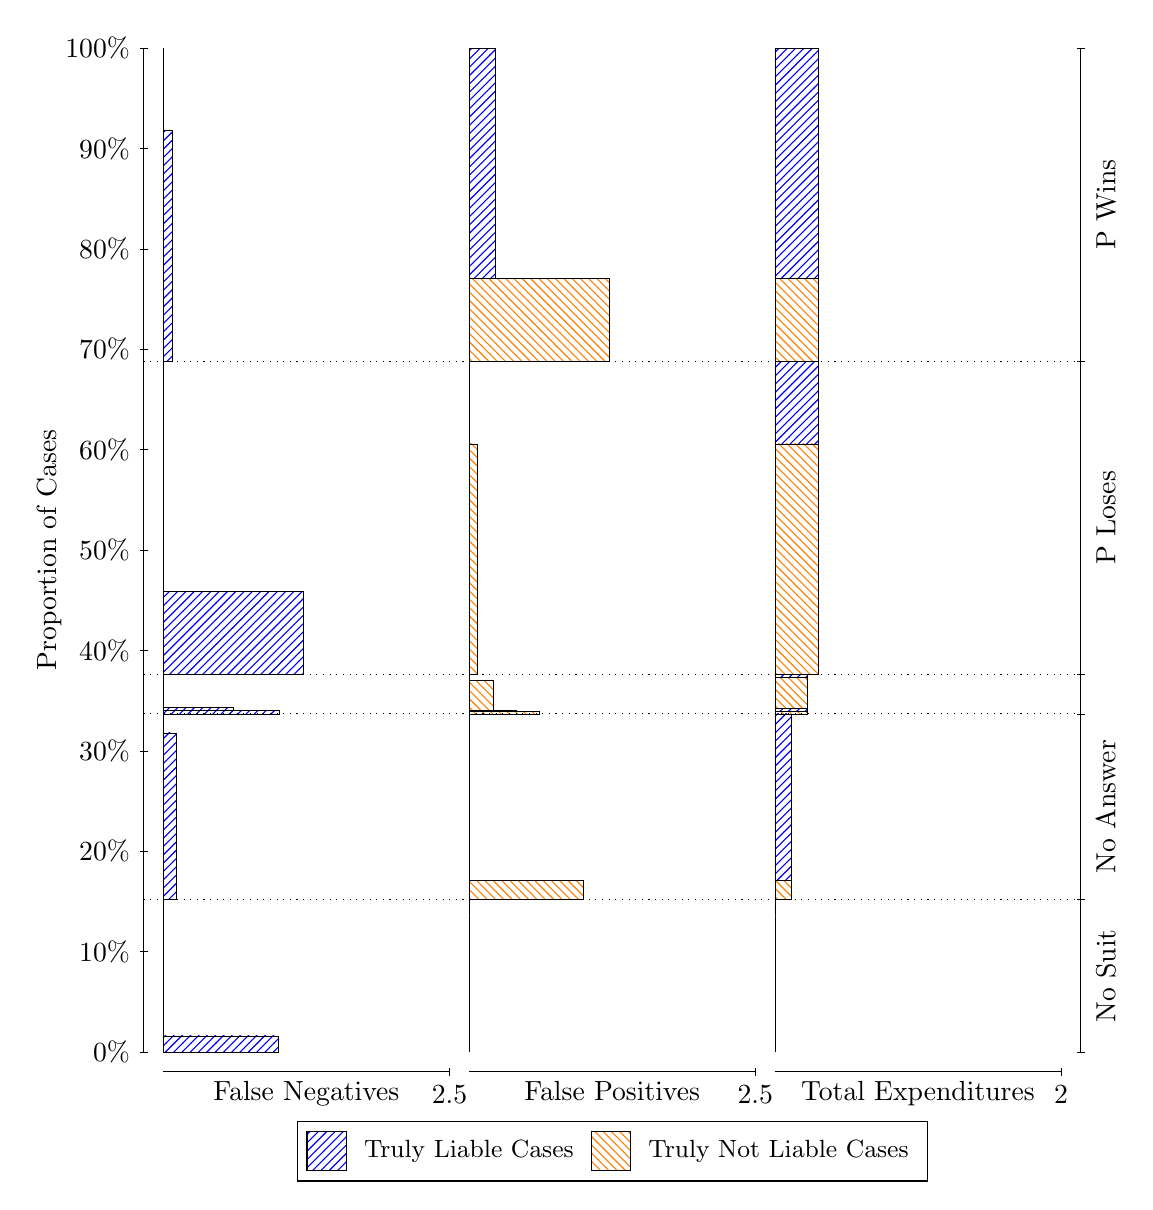
\begin{tikzpicture}
\draw[black, very thin] (1.5,1.75) -- (1.5,14.5);
\node[rotate=90, text=black, anchor=center] at (0.3, 8.125) {Proportion of Cases};
\draw[black, very thin] (1.45,1.75) -- (1.55,1.75);
\node[text=black, anchor=east] at (1.45, 1.75) {0\%};
\draw[black, very thin] (1.45,3.025) -- (1.55,3.025);
\node[text=black, anchor=east] at (1.45, 3.025) {10\%};
\draw[black, very thin] (1.45,4.3) -- (1.55,4.3);
\node[text=black, anchor=east] at (1.45, 4.3) {20\%};
\draw[black, very thin] (1.45,5.575) -- (1.55,5.575);
\node[text=black, anchor=east] at (1.45, 5.575) {30\%};
\draw[black, very thin] (1.45,6.85) -- (1.55,6.85);
\node[text=black, anchor=east] at (1.45, 6.85) {40\%};
\draw[black, very thin] (1.45,8.125) -- (1.55,8.125);
\node[text=black, anchor=east] at (1.45, 8.125) {50\%};
\draw[black, very thin] (1.45,9.4) -- (1.55,9.4);
\node[text=black, anchor=east] at (1.45, 9.4) {60\%};
\draw[black, very thin] (1.45,10.675) -- (1.55,10.675);
\node[text=black, anchor=east] at (1.45, 10.675) {70\%};
\draw[black, very thin] (1.45,11.95) -- (1.55,11.95);
\node[text=black, anchor=east] at (1.45, 11.95) {80\%};
\draw[black, very thin] (1.45,13.225) -- (1.55,13.225);
\node[text=black, anchor=east] at (1.45, 13.225) {90\%};
\draw[black, very thin] (1.45,14.5) -- (1.55,14.5);
\node[text=black, anchor=east] at (1.45, 14.5) {100\%};

\draw[black, very thin] (13.4,1.75) -- (13.4,14.5);
\draw[black, very thin] (13.35,1.75) -- (13.45,1.75);
\node[anchor=west] at (13.35, 1.75) {};
\draw[black, very thin] (13.35,3.6863) -- (13.45,3.6863);
\node[anchor=west] at (13.35, 3.6863) {};
\draw[black, very thin] (13.35,6.0446) -- (13.45,6.0446);
\node[anchor=west] at (13.35, 6.0446) {};
\draw[black, very thin] (13.35,6.5473) -- (13.45,6.5473);
\node[anchor=west] at (13.35, 6.5473) {};
\draw[black, very thin] (13.35,10.524) -- (13.45,10.524);
\node[anchor=west] at (13.35, 10.524) {};
\draw[black, very thin] (13.35,14.5) -- (13.45,14.5);
\node[anchor=west] at (13.35, 14.5) {};

\draw[black, very thin, pattern color=blue, pattern=north east lines] (1.75,1.75) rectangle (3.2033,1.9537);
\draw[black, very thin, pattern color=orange, pattern=north west lines] (1.75,1.9537) rectangle (1.75,3.6863);
\draw[black, very thin, pattern color=blue, pattern=north east lines] (1.75,3.6863) rectangle (1.9135,5.802);
\draw[black, very thin, pattern color=orange, pattern=north west lines] (1.75,5.802) rectangle (1.75,6.0446);
\draw[black, very thin, pattern color=blue, pattern=north east lines] (1.75,6.0446) rectangle (3.2215,6.0848);
\draw[black, very thin, pattern color=blue, pattern=north east lines] (1.75,6.0848) rectangle (2.9308,6.0889);
\draw[black, very thin, pattern color=blue, pattern=north east lines] (1.75,6.0889) rectangle (2.6402,6.1238);
\draw[black, very thin, pattern color=orange, pattern=north west lines] (1.75,6.1238) rectangle (1.75,6.5473);
\draw[black, very thin, pattern color=blue, pattern=north east lines] (1.75,6.5473) rectangle (3.5303,7.5977);
\draw[black, very thin, pattern color=orange, pattern=north west lines] (1.75,7.5977) rectangle (1.75,10.524);
\draw[black, very thin, pattern color=blue, pattern=north east lines] (1.75,10.524) rectangle (1.859,13.45);
\draw[black, very thin, pattern color=orange, pattern=north west lines] (1.75,13.45) rectangle (1.75,14.5);
\draw[black, very thin, pattern color=orange, pattern=north west lines] (5.6333,1.75) rectangle (5.6333,3.4826);
\draw[black, very thin, pattern color=blue, pattern=north east lines] (5.6333,3.4826) rectangle (5.6333,3.6863);
\draw[black, very thin, pattern color=orange, pattern=north west lines] (5.6333,3.6863) rectangle (7.0867,3.9289);
\draw[black, very thin, pattern color=blue, pattern=north east lines] (5.6333,3.9289) rectangle (5.6333,6.0446);
\draw[black, very thin, pattern color=orange, pattern=north west lines] (5.6333,6.0446) rectangle (6.5235,6.0795);
\draw[black, very thin, pattern color=orange, pattern=north west lines] (5.6333,6.0795) rectangle (6.2328,6.0885);
\draw[black, very thin, pattern color=orange, pattern=north west lines] (5.6333,6.0885) rectangle (5.9422,6.4681);
\draw[black, very thin, pattern color=blue, pattern=north east lines] (5.6333,6.4681) rectangle (5.6333,6.5473);
\draw[black, very thin, pattern color=orange, pattern=north west lines] (5.6333,6.5473) rectangle (5.7423,9.4733);
\draw[black, very thin, pattern color=blue, pattern=north east lines] (5.6333,9.4733) rectangle (5.6333,10.524);
\draw[black, very thin, pattern color=orange, pattern=north west lines] (5.6333,10.524) rectangle (7.4137,11.574);
\draw[black, very thin, pattern color=blue, pattern=north east lines] (5.6333,11.574) rectangle (5.9603,14.5);
\draw[black, very thin, pattern color=orange, pattern=north west lines] (9.5167,1.75) rectangle (9.5167,3.4826);
\draw[black, very thin, pattern color=blue, pattern=north east lines] (9.5167,3.4826) rectangle (9.5167,3.6863);
\draw[black, very thin, pattern color=orange, pattern=north west lines] (9.5167,3.6863) rectangle (9.721,3.9289);
\draw[black, very thin, pattern color=blue, pattern=north east lines] (9.5167,3.9289) rectangle (9.721,6.0446);
\draw[black, very thin, pattern color=orange, pattern=north west lines] (9.5167,6.0446) rectangle (9.9254,6.0795);
\draw[black, very thin, pattern color=blue, pattern=north east lines] (9.5167,6.0795) rectangle (9.9254,6.1144);
\draw[black, very thin, pattern color=orange, pattern=north west lines] (9.5167,6.1144) rectangle (9.9254,6.503);
\draw[black, very thin, pattern color=blue, pattern=north east lines] (9.5167,6.503) rectangle (9.9254,6.5473);
\draw[black, very thin, pattern color=orange, pattern=north west lines] (9.5167,6.5473) rectangle (10.062,9.4733);
\draw[black, very thin, pattern color=blue, pattern=north east lines] (9.5167,9.4733) rectangle (10.062,10.524);
\draw[black, very thin, pattern color=orange, pattern=north west lines] (9.5167,10.524) rectangle (10.062,11.574);
\draw[black, very thin, pattern color=blue, pattern=north east lines] (9.5167,11.574) rectangle (10.062,14.5);
\draw[black, dotted] (1.5,3.6863) -- (13.4,3.6863);
\draw[black, dotted] (1.5,6.0446) -- (13.4,6.0446);
\draw[black, dotted] (1.5,6.5473) -- (13.4,6.5473);
\draw[black, dotted] (1.5,10.524) -- (13.4,10.524);
\draw[black, very thin] (1.75,1.5) -- (5.3833,1.5);
\node[text=black, anchor=north] at (3.5667, 1.5) {False Negatives};
\draw[black, very thin] (5.3833,1.45) -- (5.3833,1.55);
\node[text=black, anchor=north] at (5.3833, 1.45) {2.5};

\draw[black, very thin] (5.6333,1.5) -- (9.2667,1.5);
\node[text=black, anchor=north] at (7.45, 1.5) {False Positives};
\draw[black, very thin] (9.2667,1.45) -- (9.2667,1.55);
\node[text=black, anchor=north] at (9.2667, 1.45) {2.5};

\draw[black, very thin] (9.5167,1.5) -- (13.15,1.5);
\node[text=black, anchor=north] at (11.333, 1.5) {Total Expenditures};
\draw[black, very thin] (13.15,1.45) -- (13.15,1.55);
\node[text=black, anchor=north] at (13.15, 1.45) {2};

\node[text=black, centered, rotate=90] at (13.72, 2.7182) {No Suit};
\node[text=black, centered, rotate=90] at (13.72, 4.8654) {No Answer};

\node[text=black, centered, rotate=90] at (13.72, 8.5355) {P Loses};
\node[text=black, centered, rotate=90] at (13.72, 12.512) {P Wins};

\draw (7.449999999999999,1.5) node[draw=none] (baseCoordinate) {};
\begin{scope}[align=center]
        \matrix[scale=0.5, draw=black, below=0.5cm of baseCoordinate, nodes={draw}, column sep=0.1cm]{
            \node[rectangle, draw, minimum width=0.5cm, minimum height=0.5cm, pattern color=blue, pattern=north east lines] {}; &
            \node[draw=none, font=\small, text=black] (B) {Truly Liable Cases}; &
            \node[rectangle, draw, minimum width=0.5cm, minimum height=0.5cm, pattern color=orange, pattern=north west lines] {}; &
            \node[draw=none, font=\small, text=black] (B) {Truly Not Liable Cases}; \\
            };
\end{scope}

\end{tikzpicture}
\end{document}